% Options for packages loaded elsewhere
\PassOptionsToPackage{unicode}{hyperref}
\PassOptionsToPackage{hyphens}{url}
%
\documentclass[
]{book}
\usepackage{amsmath,amssymb}
\usepackage{lmodern}
\usepackage{ifxetex,ifluatex}
\ifnum 0\ifxetex 1\fi\ifluatex 1\fi=0 % if pdftex
  \usepackage[T1]{fontenc}
  \usepackage[utf8]{inputenc}
  \usepackage{textcomp} % provide euro and other symbols
\else % if luatex or xetex
  \usepackage{unicode-math}
  \defaultfontfeatures{Scale=MatchLowercase}
  \defaultfontfeatures[\rmfamily]{Ligatures=TeX,Scale=1}
\fi
% Use upquote if available, for straight quotes in verbatim environments
\IfFileExists{upquote.sty}{\usepackage{upquote}}{}
\IfFileExists{microtype.sty}{% use microtype if available
  \usepackage[]{microtype}
  \UseMicrotypeSet[protrusion]{basicmath} % disable protrusion for tt fonts
}{}
\makeatletter
\@ifundefined{KOMAClassName}{% if non-KOMA class
  \IfFileExists{parskip.sty}{%
    \usepackage{parskip}
  }{% else
    \setlength{\parindent}{0pt}
    \setlength{\parskip}{6pt plus 2pt minus 1pt}}
}{% if KOMA class
  \KOMAoptions{parskip=half}}
\makeatother
\usepackage{xcolor}
\IfFileExists{xurl.sty}{\usepackage{xurl}}{} % add URL line breaks if available
\IfFileExists{bookmark.sty}{\usepackage{bookmark}}{\usepackage{hyperref}}
\hypersetup{
  pdftitle={Botany: A Guide for Competitive Exams},
  pdfauthor={Abhishek Kumar},
  hidelinks,
  pdfcreator={LaTeX via pandoc}}
\urlstyle{same} % disable monospaced font for URLs
\usepackage{color}
\usepackage{fancyvrb}
\newcommand{\VerbBar}{|}
\newcommand{\VERB}{\Verb[commandchars=\\\{\}]}
\DefineVerbatimEnvironment{Highlighting}{Verbatim}{commandchars=\\\{\}}
% Add ',fontsize=\small' for more characters per line
\usepackage{framed}
\definecolor{shadecolor}{RGB}{248,248,248}
\newenvironment{Shaded}{\begin{snugshade}}{\end{snugshade}}
\newcommand{\AlertTok}[1]{\textcolor[rgb]{0.94,0.16,0.16}{#1}}
\newcommand{\AnnotationTok}[1]{\textcolor[rgb]{0.56,0.35,0.01}{\textbf{\textit{#1}}}}
\newcommand{\AttributeTok}[1]{\textcolor[rgb]{0.77,0.63,0.00}{#1}}
\newcommand{\BaseNTok}[1]{\textcolor[rgb]{0.00,0.00,0.81}{#1}}
\newcommand{\BuiltInTok}[1]{#1}
\newcommand{\CharTok}[1]{\textcolor[rgb]{0.31,0.60,0.02}{#1}}
\newcommand{\CommentTok}[1]{\textcolor[rgb]{0.56,0.35,0.01}{\textit{#1}}}
\newcommand{\CommentVarTok}[1]{\textcolor[rgb]{0.56,0.35,0.01}{\textbf{\textit{#1}}}}
\newcommand{\ConstantTok}[1]{\textcolor[rgb]{0.00,0.00,0.00}{#1}}
\newcommand{\ControlFlowTok}[1]{\textcolor[rgb]{0.13,0.29,0.53}{\textbf{#1}}}
\newcommand{\DataTypeTok}[1]{\textcolor[rgb]{0.13,0.29,0.53}{#1}}
\newcommand{\DecValTok}[1]{\textcolor[rgb]{0.00,0.00,0.81}{#1}}
\newcommand{\DocumentationTok}[1]{\textcolor[rgb]{0.56,0.35,0.01}{\textbf{\textit{#1}}}}
\newcommand{\ErrorTok}[1]{\textcolor[rgb]{0.64,0.00,0.00}{\textbf{#1}}}
\newcommand{\ExtensionTok}[1]{#1}
\newcommand{\FloatTok}[1]{\textcolor[rgb]{0.00,0.00,0.81}{#1}}
\newcommand{\FunctionTok}[1]{\textcolor[rgb]{0.00,0.00,0.00}{#1}}
\newcommand{\ImportTok}[1]{#1}
\newcommand{\InformationTok}[1]{\textcolor[rgb]{0.56,0.35,0.01}{\textbf{\textit{#1}}}}
\newcommand{\KeywordTok}[1]{\textcolor[rgb]{0.13,0.29,0.53}{\textbf{#1}}}
\newcommand{\NormalTok}[1]{#1}
\newcommand{\OperatorTok}[1]{\textcolor[rgb]{0.81,0.36,0.00}{\textbf{#1}}}
\newcommand{\OtherTok}[1]{\textcolor[rgb]{0.56,0.35,0.01}{#1}}
\newcommand{\PreprocessorTok}[1]{\textcolor[rgb]{0.56,0.35,0.01}{\textit{#1}}}
\newcommand{\RegionMarkerTok}[1]{#1}
\newcommand{\SpecialCharTok}[1]{\textcolor[rgb]{0.00,0.00,0.00}{#1}}
\newcommand{\SpecialStringTok}[1]{\textcolor[rgb]{0.31,0.60,0.02}{#1}}
\newcommand{\StringTok}[1]{\textcolor[rgb]{0.31,0.60,0.02}{#1}}
\newcommand{\VariableTok}[1]{\textcolor[rgb]{0.00,0.00,0.00}{#1}}
\newcommand{\VerbatimStringTok}[1]{\textcolor[rgb]{0.31,0.60,0.02}{#1}}
\newcommand{\WarningTok}[1]{\textcolor[rgb]{0.56,0.35,0.01}{\textbf{\textit{#1}}}}
\usepackage{longtable,booktabs,array}
\usepackage{calc} % for calculating minipage widths
% Correct order of tables after \paragraph or \subparagraph
\usepackage{etoolbox}
\makeatletter
\patchcmd\longtable{\par}{\if@noskipsec\mbox{}\fi\par}{}{}
\makeatother
% Allow footnotes in longtable head/foot
\IfFileExists{footnotehyper.sty}{\usepackage{footnotehyper}}{\usepackage{footnote}}
\makesavenoteenv{longtable}
\usepackage{graphicx}
\makeatletter
\def\maxwidth{\ifdim\Gin@nat@width>\linewidth\linewidth\else\Gin@nat@width\fi}
\def\maxheight{\ifdim\Gin@nat@height>\textheight\textheight\else\Gin@nat@height\fi}
\makeatother
% Scale images if necessary, so that they will not overflow the page
% margins by default, and it is still possible to overwrite the defaults
% using explicit options in \includegraphics[width, height, ...]{}
\setkeys{Gin}{width=\maxwidth,height=\maxheight,keepaspectratio}
% Set default figure placement to htbp
\makeatletter
\def\fps@figure{htbp}
\makeatother
\setlength{\emergencystretch}{3em} % prevent overfull lines
\providecommand{\tightlist}{%
  \setlength{\itemsep}{0pt}\setlength{\parskip}{0pt}}
\setcounter{secnumdepth}{5}
\usepackage{booktabs}
\usepackage{amsthm}
\makeatletter
\def\thm@space@setup{%
  \thm@preskip=8pt plus 2pt minus 4pt
  \thm@postskip=\thm@preskip
}
\makeatother
\ifluatex
  \usepackage{selnolig}  % disable illegal ligatures
\fi
\usepackage[]{natbib}
\bibliographystyle{apalike}

\title{Botany: A Guide for Competitive Exams}
\author{Abhishek Kumar}
\date{2021-03-21}

\begin{document}
\maketitle

{
\setcounter{tocdepth}{1}
\tableofcontents
}
\hypertarget{preface}{%
\chapter*{Preface}\label{preface}}
\addcontentsline{toc}{chapter}{Preface}

This is a \emph{sample} book written in \textbf{Markdown}. You can use anything that Pandoc's Markdown supports, e.g., a math equation \(a^2 + b^2 = c^2\).

The \textbf{bookdown} package can be installed from CRAN or Github:

\begin{Shaded}
\begin{Highlighting}[]
\FunctionTok{install.packages}\NormalTok{(}\StringTok{"bookdown"}\NormalTok{)}
\CommentTok{\# or the development version}
\CommentTok{\# devtools::install\_github("rstudio/bookdown")}
\end{Highlighting}
\end{Shaded}

Remember each Rmd file contains one and only one chapter, and a chapter is defined by the first-level heading \texttt{\#}.

To compile this example to PDF, you need XeLaTeX. You are recommended to install TinyTeX (which includes XeLaTeX): \url{https://yihui.name/tinytex/}.

\hypertarget{about-the-author}{%
\chapter*{About the Author}\label{about-the-author}}
\addcontentsline{toc}{chapter}{About the Author}

\href{https://akumar.netlify.app/}{Abhishek Kumar} is a senior research fellow at the Soil Ecosystem and Restoration Ecology Lab in the Department of Botany, Panjab University, Chandigarh. His research interests include the responses of ecological structure and functions to climate change, and he is currently working on the elevational pattern of plant distributions and diversity in the Siwalik Ecosystem.

\hypertarget{intro}{%
\chapter{Introduction}\label{intro}}

You can label chapter and section titles using \texttt{\{\#label\}} after them, e.g., we can reference Chapter \ref{intro}. If you do not manually label them, there will be automatic labels anyway, e.g., Chapter \ref{methods}.

Figures and tables with captions will be placed in \texttt{figure} and \texttt{table} environments, respectively.

\begin{Shaded}
\begin{Highlighting}[]
\FunctionTok{par}\NormalTok{(}\AttributeTok{mar =} \FunctionTok{c}\NormalTok{(}\DecValTok{4}\NormalTok{, }\DecValTok{4}\NormalTok{, .}\DecValTok{1}\NormalTok{, .}\DecValTok{1}\NormalTok{))}
\FunctionTok{plot}\NormalTok{(pressure, }\AttributeTok{type =} \StringTok{\textquotesingle{}b\textquotesingle{}}\NormalTok{, }\AttributeTok{pch =} \DecValTok{19}\NormalTok{)}
\end{Highlighting}
\end{Shaded}

\begin{figure}

{\centering 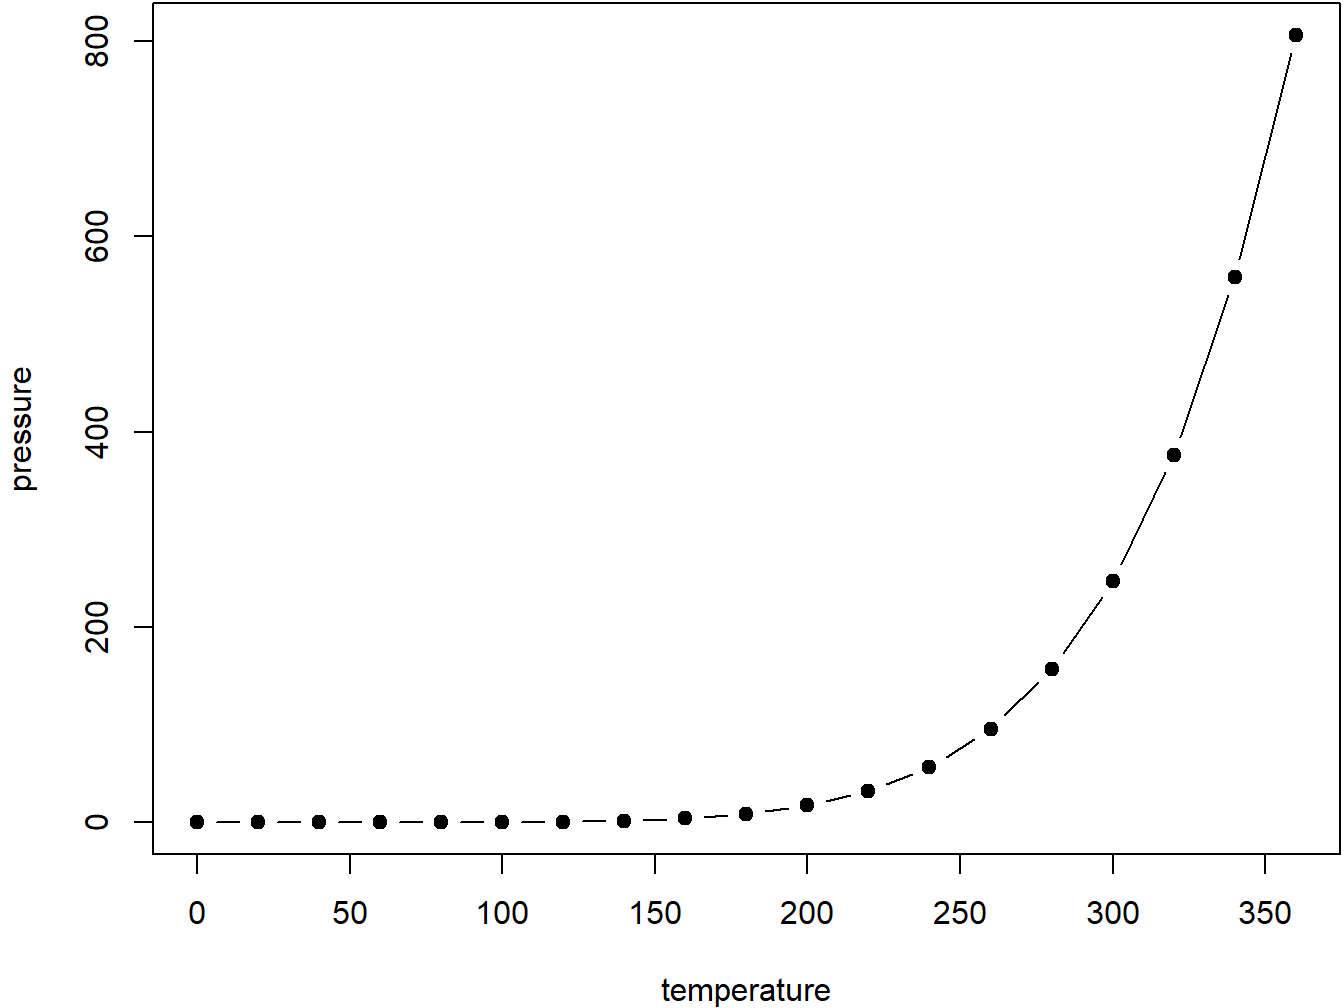
\includegraphics[width=0.8\linewidth]{bookdown-demo_files/figure-latex/nice-fig-1} 

}

\caption{Here is a nice figure!}\label{fig:nice-fig}
\end{figure}

Reference a figure by its code chunk label with the \texttt{fig:} prefix, e.g., see Figure \ref{fig:nice-fig}. Similarly, you can reference tables generated from \texttt{knitr::kable()}, e.g., see Table \ref{tab:nice-tab}.

\begin{Shaded}
\begin{Highlighting}[]
\NormalTok{knitr}\SpecialCharTok{::}\FunctionTok{kable}\NormalTok{(}
  \FunctionTok{head}\NormalTok{(iris, }\DecValTok{20}\NormalTok{), }\AttributeTok{caption =} \StringTok{\textquotesingle{}Here is a nice table!\textquotesingle{}}\NormalTok{,}
  \AttributeTok{booktabs =} \ConstantTok{TRUE}
\NormalTok{)}
\end{Highlighting}
\end{Shaded}

\begin{table}

\caption{\label{tab:nice-tab}Here is a nice table!}
\centering
\begin{tabular}[t]{rrrrl}
\toprule
Sepal.Length & Sepal.Width & Petal.Length & Petal.Width & Species\\
\midrule
5.1 & 3.5 & 1.4 & 0.2 & setosa\\
4.9 & 3.0 & 1.4 & 0.2 & setosa\\
4.7 & 3.2 & 1.3 & 0.2 & setosa\\
4.6 & 3.1 & 1.5 & 0.2 & setosa\\
5.0 & 3.6 & 1.4 & 0.2 & setosa\\
\addlinespace
5.4 & 3.9 & 1.7 & 0.4 & setosa\\
4.6 & 3.4 & 1.4 & 0.3 & setosa\\
5.0 & 3.4 & 1.5 & 0.2 & setosa\\
4.4 & 2.9 & 1.4 & 0.2 & setosa\\
4.9 & 3.1 & 1.5 & 0.1 & setosa\\
\addlinespace
5.4 & 3.7 & 1.5 & 0.2 & setosa\\
4.8 & 3.4 & 1.6 & 0.2 & setosa\\
4.8 & 3.0 & 1.4 & 0.1 & setosa\\
4.3 & 3.0 & 1.1 & 0.1 & setosa\\
5.8 & 4.0 & 1.2 & 0.2 & setosa\\
\addlinespace
5.7 & 4.4 & 1.5 & 0.4 & setosa\\
5.4 & 3.9 & 1.3 & 0.4 & setosa\\
5.1 & 3.5 & 1.4 & 0.3 & setosa\\
5.7 & 3.8 & 1.7 & 0.3 & setosa\\
5.1 & 3.8 & 1.5 & 0.3 & setosa\\
\bottomrule
\end{tabular}
\end{table}

You can write citations, too. For example, we are using the \textbf{bookdown} package \citep{R-bookdown} in this sample book, which was built on top of R Markdown and \textbf{knitr} \citep{xie2015}.

\hypertarget{part-biochemistry}{%
\part{Biochemistry}\label{part-biochemistry}}

\hypertarget{biomolecules}{%
\chapter{Biomolecules}\label{biomolecules}}

The most exciting aspect of chemistry deal with isolating thousands of compounds, small and big, from living organisms, determining their structure and if possible, synthesizing them. If one were to make a list of biomolecules, such a list would have thousands of organic compounds including amino acids, sugars, etc. We can call these biomolecules, metabolites. In animal tissues, one notices the presence of all such categories of compounds e.g., proteins, carbohydrates, fats, amino acids and nucleic acids. These are called primary metabolites. However, when one analyses plant, fungal and microbial cells, one would see thousands of compounds other than these primary metabolites e.g., alkaloids, flavonoids, rubber, essential oils, antibiotics, coloured pigments, scents, gums, spices, etc. These are called secondary metabolites (Table \ref{tab:t1}). While primary metabolites have identifiable functions and play known roles in normal physiological processes, many secondary metabolites are useful to `human welfare' (e.g., rubber, drugs, spices, scents and pigments). Some secondary metabolites have ecological importance.

\begin{longtable}[]{@{}ll@{}}
\caption{\textbf{\label{tab:t1} Some Secondary Metabolites}}\tabularnewline
\toprule
Secondary Metabolites & Examples \\
\midrule
\endfirsthead
\toprule
Secondary Metabolites & Examples \\
\midrule
\endhead
Pigments & Carotenoids, Anthocyanins, etc. \\
Alkaloids & Morphine, Codeine, etc. \\
Terpenoids & Monoterpenes, Diterpenes, etc. \\
Essential oils & Lemon grass oil, etc. \\
Toxins & Abrin, Ricin \\
Lectins & Concanavalin \\
Polymeric substances & Rubber, Gums, Cellulose \\
Drugs & Vinblastine, curcumin, etc. \\
\bottomrule
\end{longtable}

In both the cells and extra-cellular fluids dibasic phosphate (HPO\textsubscript{4}\textsuperscript{2-}) and monobasic phosphate (H\textsubscript{2}PO\textsubscript{4}\textsuperscript{--}) neutralise strong acids and bases respectively. So, they act as acid-base buffers to maintain the H+ ion concentration (pH) of cellular fluids. All the macromolecules except lipids are formed by the process of polymerisation, a process in which repeating sub-units termed monomers are bound into chains of different length (Polymers) e.g., Raffinose is trisaccharide formed by polymerisation of glucose, fructose and galactose.

\hypertarget{carbohydrates}{%
\section{Carbohydrates}\label{carbohydrates}}

Carbohydrates are so called because in most of them, the proportion of hydrogen and oxygen is the same as in water (H\textsubscript{2}O) and the general formula may be written as C\textsubscript{n}H\textsubscript{2n}O\textsubscript{n}. Carbohydrates also possess more than one alcoholic (OH) group.
Carbohydrates are known as saccharides or compounds containing sugar. The simplest carbohydrates are the simple sugars or monosaccharides, many of which have the general formula C\textsubscript{n}H\textsubscript{2n}O\textsubscript{n}. These cannot be hydrolysed into still smaller carbohydrates. Monosaccharides are composed of 3 to 7 carbon atoms. They are classified according to the number of carbon atoms, as trioses (C\textsubscript{3}H\textsubscript{6}O\textsubscript{3}), tetroses (C\textsubscript{4}H\textsubscript{8}O\textsubscript{4}), pentoses (C\textsubscript{5}H\textsubscript{10}O\textsubscript{5}), hexoses (C\textsubscript{6}H\textsubscript{12}O\textsubscript{6}) and heptoses (C\textsubscript{7}H\textsubscript{14}O\textsubscript{7}) in that order. Hexoses and pentoses exist in both open chain and ring forms. Glucose, fructose and galactose are hexoses. They are all white, crystalline, sweet-tasting substances, extremely soluble in water. Ribose is a pentose and glyceraldehyde and dihydroxyacetone are trioses. These compounds have very important roles to play in the metabolism of cells as you will learn later. Glucose is the most important sugar occurring in animals. Fructose is the commonest form of sugar in fruits. Deoxyribose which occurs in deoxyribonucleic acid (DNA) is a pentose.

\hypertarget{methods}{%
\chapter{Methods}\label{methods}}

We describe our methods in this chapter.

\hypertarget{applications}{%
\chapter{Applications}\label{applications}}

Some \emph{significant} applications are demonstrated in this chapter.

\hypertarget{example-one}{%
\section{Example one}\label{example-one}}

\hypertarget{example-two}{%
\section{Example two}\label{example-two}}

\hypertarget{final-words}{%
\chapter{Final Words}\label{final-words}}

We have finished a nice book.

\hypertarget{part-diversity}{%
\part{Diversity}\label{part-diversity}}

\hypertarget{biological-classification}{%
\chapter{Biological Classification}\label{biological-classification}}

\hypertarget{the-living-world}{%
\section{The Living World}\label{the-living-world}}

Life is a unique, complex organisation of molecules expressing itself through chemical reactions which lead to growth development responsiveness, adaptation and reproduction. Life is recognised by mode of its working which includes some unified and basic characteristics. The important characteristics are:

\begin{enumerate}
\def\labelenumi{\arabic{enumi}.}
\item
  \textbf{Growth:} All living beings grow. Increase in mass and increase in number of cells are twin characters of growth. In unicellular organisms, it can be increase in size and mass, whereas in multicellular, it is increase in the number of cells. The growth takes place by cell division. In plants, the growth by cell division occurs continuously throughout their life span and therefore, is indefinite, whereas in animals this growth is seen only up to a certain age and hence it is definite. Non-living objects also grow if we take increase in body mass as a criterion of growth. Growth therefore, cannot be taken as a defining property of living organisms.
\item
  \textbf{Reproduction:} The reproduction means to produce progeny possessing features more or less similar to those of the parents. The organisms can reproduce asexually as well as sexually. There are different methods of asexual reproduction in different forms of organisms. Reproduction is synonymous with growth in unicellular organisms i.e., increase in the number of cells is equivalent to reproduction. Further, there are some organisms which do not reproduce at all e.g., Worker bees, mules. Hence, reproduction also cannot be an all-inclusive property of living organisms.
\item
  \textbf{Metabolism:} All living beings show metabolism. It is defined as sum total of all chemical reactions taking place in the body of an organism. Some of the chemical reactions are constructive and are called as anabolic, whereas others are destructive and are called as catabolic. If anabolism exceeds catabolism, growth takes place.
\item
  \textbf{Irritability:} All living beings respond to the external stimuli. The response given by an organism to the stimulus is called as Irritability. It Is because of presence of either nervous system or some sensory structures in different forms of life. Thus, consciousness is defining property
\end{enumerate}

\hypertarget{systematics-and-taxonomy}{%
\section{Systematics and Taxonomy}\label{systematics-and-taxonomy}}

\hypertarget{diversity-of-life}{%
\subsection{Diversity of Life}\label{diversity-of-life}}

The variety of living organisms on Earth, including plants, animals, bacteria, and fungi, is enormous \citep{mora2011}.

\begin{itemize}
\tightlist
\item
  Predicted number of total species on earth is 5 to 50 million. Average number is 14 million.
\item
  It is estimated that there are perhaps 10 million eukaryotic species and an unknown number of prokaryotic ones \citep{mora2011}.
\item
  According to \href{https://www.catalogueoflife.org/}{Catalogue of Life} Number of taxonomically known species is over 1.83 million.
\item
  These include nearly 1.2 million animals and over 0.5 million species of plants. Amongst animals, insects form the largest group i.e., over 10,25,000 species. Every year known or discovered number of species is 15,000.
\end{itemize}

\hypertarget{need-of-classification}{%
\subsection{Need of Classification}\label{need-of-classification}}

Keeping in view vast diversity of living organism, there is a need to classify organisms.

\begin{itemize}
\tightlist
\item
  Gives an idea about diversity of organisms
\item
  Throws light into the origin of organisms
\item
  Gives information about evolutionary Interrelations between organisms
\item
  By studying one member of a group, a broad idea regarding all organisms of the group can be obtained
\end{itemize}

\hypertarget{systematics}{%
\subsection{Systematics}\label{systematics}}

The scientific study of this biological diversity and its evolutionary history is called \textbf{systematics}.

\begin{figure}
\centering
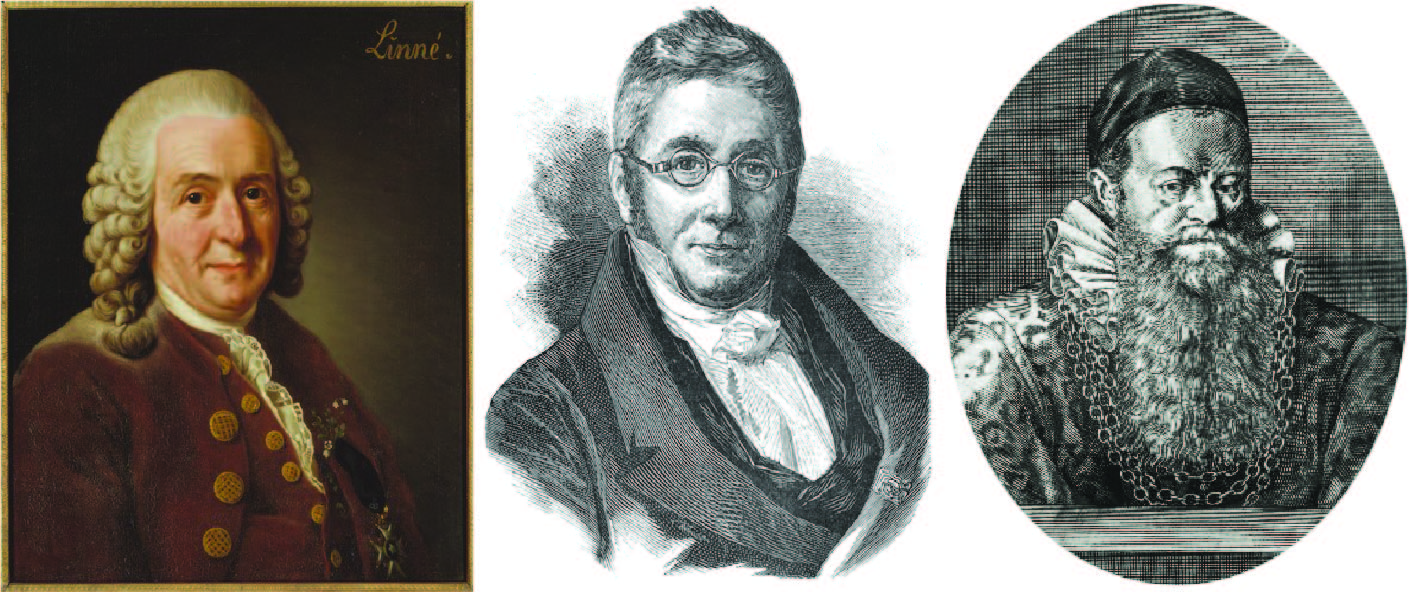
\includegraphics{images/workers.jpg}
\caption{\label{fig:fig1} Carl Linnaeus, A. P. de Candolle and C. Bauhin (left to right)}
\end{figure}

\begin{itemize}
\tightlist
\item
  Term given by \href{https://en.wikipedia.org/wiki/Carl_Linnaeus}{Carolus Linnaeus} (Figure \ref{fig:fig1})
\item
  Study of diversity of organisms and their comparative and evolutionary relationship.
\item
  Systematics = Taxonomy + Phylogeny
\item
  \textbf{Phylogeny} is the evolutionary history of organisms
\item
  Most of the taxonomist believed that both taxonomy and systematics are interchangeable, but \textbf{G. Simpson} considered these as separate fields.
\end{itemize}

\hypertarget{taxonomy}{%
\subsection{Taxonomy}\label{taxonomy}}

\begin{itemize}
\tightlist
\item
  Term by \href{https://en.wikipedia.org/wiki/Augustin_Pyramus_de_Candolle}{A. P. de Candolle} (Figure \ref{fig:fig1}) -- in his book \href{https://www.biodiversitylibrary.org/bibliography/39705}{\emph{Theorie Elementaire de la Botanique}}.
\item
  Study of principles and procedures of classification of organisms
\item
  Components of taxonomy are Characterisation, Identification, Nomenclature and Classification
\item
  Identification is the first step of taxonomy, and is based upon characterisation
\end{itemize}

\hypertarget{taxonomic-hierarchy}{%
\subsection{Taxonomic Hierarchy}\label{taxonomic-hierarchy}}

The placement of organisms to different ranks in a systematic framework of classification. This framework is called taxonomic hierarchy.

\begin{itemize}
\tightlist
\item
  First given by Linnaeus who introduced 5 ranks i.e.,\\
  Class --- order --- genus --- species --- variety (from upper to lower)
\item
  Later on, modified with 7 obligate categories and about 21 intermediate categories. Seven obligate categories are:\\
  Kingdom---Phylum/Division---Class---Order---Family---Genus---Species (from higher to lower)
\item
  Domain---Kingdom---Phylum/Division---Class---Order---Family---Genus---Species \textcolor{red}{[ICFRE 2020]}
\item
  Higher the category; higher the number of organisms and lesser the number of common characters.\\
\item
  Intermediate categories are written with prefix `super' and `sub', e.g., superclass; subclass. Intraspecies categories (Intermediate categories)\\
  Sub-species/varieties---subvariety---form/race---subform or clone
\end{itemize}

\begin{longtable}[]{@{}ll@{}}
\caption{\textbf{\label{tab:term-author} Terms and their Authors}}\tabularnewline
\toprule
Term (s) & Author \\
\midrule
\endfirsthead
\toprule
Term (s) & Author \\
\midrule
\endhead
Phylum & Cuvier \\
Division & Eichler \\
Class, Order & Linnaeus \\
Family, Species & John Ray \\
Genus & Toumefort \\
Concept of Genus & Brunfels \\
\bottomrule
\end{longtable}

\begin{itemize}
\tightlist
\item
  Taxon is a taxonomic group of real organisms assigned to a category. Category represents rank/level in a hierarchy
\end{itemize}

\hypertarget{species-concept-and-types}{%
\section{Species Concept and Types}\label{species-concept-and-types}}

\hypertarget{species-concept}{%
\subsection{Species Concept}\label{species-concept}}

Species concepts \citep{dequeiroz2007}

\begin{enumerate}
\def\labelenumi{\arabic{enumi}.}
\item
  \textbf{Morphological/Static/Typological Concept:} By Linnaeus; Species are fixed, Immutable and can be recognised by their morphological features.
\item
  \textbf{Dynamic Concept of Species:} By Lamarck; Mutable and Changeable
\item
  \textbf{Biological Concept of Species:} By Ernst Mayr; Based on reproductive Isolation. K. Jordan (1905) first gave the definition, Later Mayr proposed the biological species concept. According to this concept, \emph{``a species is a group of interbreeding natural population that is reproductively isolated from other such groups''}. Exceptions of ``Biological Concept of Species'' / Reproductive isolation:
\end{enumerate}

\begin{longtable}[]{@{}ll@{}}
\caption{\textbf{\label{tab:hybridisation-type} Exceptions to Biological Concept of Species}}\tabularnewline
\toprule
Hybridisation & Reproductive Potential \\
\midrule
\endfirsthead
\toprule
Hybridisation & Reproductive Potential \\
\midrule
\endhead
♂ Donkey × ♀ Horse = Mule & Sterile hybrids (under natural conditions) \\
♂ Horse × ♀ Donkey = Hinny & Sterile hybrids (under natural conditions) \\
♂ Tiger × ♀ Lion = Tigon & Fertile hybrids (under captive conditions) \\
♂ Lion × ♀ Tiger = Liger & Fertile hybrids (under captive conditions) \\
\bottomrule
\end{longtable}

\begin{enumerate}
\def\labelenumi{\arabic{enumi}.}
\setcounter{enumi}{3}
\tightlist
\item
  \textbf{Evolutionary Species Concept:} Simpson (1961) has proposed that \emph{``an evolutionary species is a lineage (an ancestral- descendant sequence of populations) evolving separately from others and with its own unitary evolutionary role and tendencies''}. Christoffersen (1995) proposed the \textbf{ontological species concept} that is \emph{``a species is a single lineage of ancestral descendant sexual populations genetically integrated by historically contingent events of interbreeding''}. This definition of Christoffersen has given stress on the interbreeding nature of a species.
\end{enumerate}

\hypertarget{species-types}{%
\subsection{Species Types}\label{species-types}}

\begin{longtable}[]{@{}
  >{\raggedright\arraybackslash}p{(\columnwidth - 2\tabcolsep) * \real{0.21}}
  >{\raggedright\arraybackslash}p{(\columnwidth - 2\tabcolsep) * \real{0.79}}@{}}
\caption{\textbf{\label{tab:species-type} Major types of Species}}\tabularnewline
\toprule
Species Type & Description \\
\midrule
\endfirsthead
\toprule
Species Type & Description \\
\midrule
\endhead
Morphospecies & Species erected on the basis of morphological characters \\
Taxonomic species & Species with binomial name \\
Sibling species & Two different species which are morphologically identical but do not interbreed \\
Allopatric species & Species having, exclusive area of geographical distribution \\
Sympatric species & Species having overlapping areas of geographical distribution \\
Parapatric species & Species found in narrow overlapping zone \\
Allochronic species & Species belonging to different time period \\
Synchronic species & Species belonging to same time period \\
\bottomrule
\end{longtable}

\hypertarget{nomenclature}{%
\section{Nomenclature}\label{nomenclature}}

\textbf{Vernacular names} are the names given in local language, which varies from place to place and language to language. Thus, these names are not universal. On the other hand, \textbf{Scientific names} give a universal name to a particular organism on the basis of definite rules and criteria.

\begin{enumerate}
\def\labelenumi{\arabic{enumi}.}
\item
  \textbf{Polynomial nomenclature:} Introduced before 1750, organism's name consists of a series of latinised descriptive words. Such names became lengthy and difficult to learn. e.g., \emph{Caryophyllum saxatilis folis gramineus umbellatis corymbis}. For example, for catnip, which was formally named \emph{Nepeta floribus interrupte spicatus pedunculatis} (meaning ``\emph{Nepeta} with flowers in an interrupted pedunculate spike'').
\item
  \textbf{Binomial nomenclature:}
\end{enumerate}

\begin{itemize}
\tightlist
\item
  First proposed by \href{https://en.wikipedia.org/wiki/Gaspard_Bauhin}{Gaspard Bauhin} (or Caspar Bauhin) in \href{https://bibdigital.rjb.csic.es/idurl/1/10754}{\emph{Pinax Theatri Botanici (1623)}}
\item
  Introduced by Carolus Linnaeus; Swedish naturalist who changed his name according to binomial nomenclature. His old name was Karl Von Linne.
\item
  Organism's name consists of two Latin words. First name is generic and second name is species epithet. e.g., Garden pea -- \emph{Pisum sativum} (L). Letter in bracket shows the name of scientist who gave the name.
\item
  Binomial epithet = genus + species + author's citation
\item
  Linnaeus gave some principles of the binomial nomenclature in \emph{Philosophia Botanica}, But the nomenclature was use first in \emph{Species Plantarum}, where names and description of 5,900 species of plants were given. Later he published \emph{Systema Naturae}, where 4,326 species of a were described.
\end{itemize}

\begin{enumerate}
\def\labelenumi{\arabic{enumi}.}
\setcounter{enumi}{2}
\tightlist
\item
  \textbf{Trinomial nomenclature:}
\end{enumerate}

\begin{itemize}
\tightlist
\item
  Given by \textbf{Lamarck}, it consists of 3 words i.e., genus + species + sub-species or varieties (Table \ref{tab:t71}).
\item
  In animal kingdom - third name is subspecies whereas in plantae - it is varieties.
\end{itemize}

\begin{longtable}[]{@{}ll@{}}
\caption{\textbf{\label{tab:t71} Examples of Trinomial Nomenclature}}\tabularnewline
\toprule
Vernacular Name & Scientific Name \\
\midrule
\endfirsthead
\toprule
Vernacular Name & Scientific Name \\
\midrule
\endhead
Indian crow & \emph{Corvus splendens splendens} \\
Srilankan crow & \emph{Corvus splendens protegatus} \\
Bunnese crow & \emph{Corvus splendens insolens} \\
Cabbage & \emph{Brassica oleracea capitata} \\
\bottomrule
\end{longtable}

\hypertarget{standardisation-of-names}{%
\subsection{Standardisation of Names}\label{standardisation-of-names}}

\begin{itemize}
\tightlist
\item
  ICBN (1961): International Code of Botanical Nomenclature (Earlier)
\item
  ICNafp (2018): International Code of Nomenclature for Algae, Fungi, and Plants \textcolor{red}{[ICFRE 2020; CGPSC 2020]}
\item
  ICZN (1964): International Code of Zoological Nomenclature
\item
  ICNB: International Code for Nomenclature of Bacteria
\item
  ICNCP: International Code of Nomenclature for Cultivated Plants
\item
  ICTV: International Committee for the Taxonomy of Virus
\end{itemize}

\hypertarget{terminology}{%
\subsection{Terminology}\label{terminology}}

\begin{itemize}
\tightlist
\item
  \textbf{Tautonyms:} An organism with same generic and species name. It is not applicable in plants. e.g., \emph{Rattus rattus}.
\item
  \textbf{Autonyms:} When species and subspecies names are same. e.g., \emph{Corvus splendens splendens}.
\item
  \textbf{Synonyms:} When two or more names are given, the first name is recognised as valid name and all other names are called synonyms. e.g., \emph{Albugo candida} (valid name); \emph{Cystopus candidus} (synonym).
\item
  \textbf{Homonyms:} One name for two different plants. e.g., \emph{Prunus dulsi} (almond and plum).
\end{itemize}

\hypertarget{nomenclatural-types}{%
\subsection{Nomenclatural Types}\label{nomenclatural-types}}

\begin{longtable}[]{@{}
  >{\raggedright\arraybackslash}p{(\columnwidth - 2\tabcolsep) * \real{0.09}}
  >{\raggedright\arraybackslash}p{(\columnwidth - 2\tabcolsep) * \real{0.91}}@{}}
\caption{\textbf{\label{tab:t72} Nomenclatural Types}}\tabularnewline
\toprule
Type & Description \\
\midrule
\endfirsthead
\toprule
Type & Description \\
\midrule
\endhead
Holotype & Nomenclature type \\
Isotype & Duplicate of holotype \\
Paratype & Any other specimen described along with holotype \\
Syntype & Any one of the two or more specimens cited by author when there is no holotype \\
Lectotype & Specimen selected from original material to serve as nomenclature type where there is no holotype (missing) \\
Neotype & New nomenclature type when the original material is missing \\
Topotype & It is name given to a specimen collected from the same locality from which the holotype was originally collected \\
\bottomrule
\end{longtable}

\hypertarget{taxonomic-literature}{%
\section{Taxonomic Literature}\label{taxonomic-literature}}

According to Porter (1967) \emph{``Taxonomic literature runs the gamut from ponderous volumes to obscure notes in periodicals and even letters of correspondence between workers''}.

\begin{enumerate}
\def\labelenumi{\arabic{enumi}.}
\item
  \textbf{Classics:} The works which have been profoundly influenced the development of plant taxonomy and regarded as landmarks in the history of Botany are called Classics. They include the works of Theophrastus, Pliny, Dioscorides, Albertus Magnus, Brunfels, Cesalpino, the Bauhins, Ray, Tournefort and Linnaeus.
\item
  \textbf{Taxonomic Indexes:} The taxonomic indexes are indexes of plant names and not to literature concerning the plants. Indexes serve as an aid to locating quickly the source of original publication of a name, to learn if a particular name has been applied to a plant or to what order, family, subfamily or tribe, a plant of a given name may belong. These indexes are the nucleus of any significant taxonomic library, and it is incumbent on the student of taxonomy to know of their availability and importance. Important taxonomic indices are:

  \begin{enumerate}
  \def\labelenumii{\roman{enumii})}
  \tightlist
  \item
    \href{https://naturalhistory2.si.edu/botany/ing/}{\emph{Index Nominum Genericorum} (ING)}: A compilation of generic names published for organisms covered by the ICN: International Code of Nomenclature for Algae, Fungi, and Plants. It is the list of all generic names of plants of all groups (Fossil and Recent). It was published by E.R. Far, J. A. Leussinke and F. A. Stfleu in 1979 in 3 volumes. It included all generic names from 1753 to 1975.
  \item
    \href{https://www.biodiversitylibrary.org/openurlmultiple.aspx?id=p42382218\%7Cp42403161\%7Cp42462730\%7Cp42402499}{\emph{Index Kewensis Plantarum Phanerogamarun} (IK)}: Generally called \emph{Index Kewensis} (IK). It is the most comprehensive list of scientific names of seed plants (Gymnosperms and Angiosperms). The first 2 volumes were compiled by J.D. Hooker and B.D. Jackson in 1893-1895 at Kew. It includes generic names in alphabetical order between 1753-1885.
  \item
    \href{https://www.ipni.org/}{\emph{International Plant Name Index} (IPNI)}:
  \item
    \href{http://sweetgum.nybg.org/science/ih/}{\emph{Index Herbariorum}}: It is a guide to the location and contents of the world's public herbaria.
  \end{enumerate}
\item
  \textbf{Floras:} A flora is a systematic arrangement of the species of a given area or a particular region, usually restricted to a major segment of the plant kingdom (flowering plants etc.), with keys and descriptions and often illustrations, by the use of which a student may determine the names and characteristics of the wild plants of the area. In any flora the plants are arranged according to one or another of the available systems (Engler, Bessey, Hutchinson, etc.), giving for each plant the complete scientific name, author citation, reference to source of original publication, synonymy, and geographic distribution within the area in question.
\item
  \textbf{Monographs and Revisions:} A monograph is a treatise including all significant information of a morphologic or taxonomic nature covering the group such as family or genus. A taxonomic monograph is a comprehensive treatise representing an analysis and synthesis of existing taxonomic knowledge of that taxon, plus the results of original research of that in systematics. In other words, it is ``as complete an account as can be made at a given time of any one family, tribe, or genus, 'nothing being neglected which is necessary for a perfect knowledge of it.'' A taxonomic revision differs from a monograph primarily in degree of scope and completeness. Often it accounts for only a section of a genus or for the elements as restricted to a continent or smaller geographical area. Many revisions make no attempt to review all previous work on the taxon or to take cognizance of the interrelated sciences of cytotaxonomy, genetics, ecology, etc. A revision may be based only on herbarium studies, where as monograph should cover the morphology, anatomy, cytology, genetics and ecology.
\item
  \textbf{Catalogues:} Catalogues account for the books of special libraries rich in botanical titles, and are of especial value in taxonomic studies. It is often necessary to know the full name of a particular author, to know the unabridged and exact title of a work, to know when it was published, or when a particular edition was issued. These data are usually available from such catalogues.
\item
  \textbf{Review Serials:} Review serials are periodicals, usually issued at regular intervals, that provide either:

  \begin{enumerate}
  \def\labelenumii{\roman{enumii})}
  \tightlist
  \item
    A bibliography of current literature of a particular subject,
  \item
    An abstract of papers or books in special fields,
  \item
    Reviews of titles of current literature, or
  \item
    Any combination of these functions.
  \end{enumerate}
\item
  \textbf{Periodical:} A periodical, is a publication appearing usually at regular intervals. Each issue is called a number, or sometimes is termed a fascicle. Collectively these numbers or fascicles comprise a volume. In the case of periodicals appearing at regular intervals -- biweekly, monthly, or quarterly- a volume usually comprises the issues of a calendar year.
\item
  \textbf{Dictionaries and Glossaries:} Dictionaries and glossaries from the nucleus of taxonomic literature. Dictionaries and glossaries are invaluable in a subject matter with so large a vocabulary as that of Botany. A botanical dictionary may list and describe all known genera of certain plant groups e.g.~A Dictionary of Flowering, Plants and Ferns by J. C. Willis. A glossary is an alphabetical list of difficult terms with their interpretations.
\end{enumerate}

\hypertarget{important-contributions-of-linnaeus}{%
\subsection{Important Contributions of Linnaeus}\label{important-contributions-of-linnaeus}}

\begin{itemize}
\item
  Father of Taxonomy
\item
  Binomial Nomenclature
\item
  Artificial System of Classification
\item
  \emph{Species Plantarum} (1753): It was published in 2 volumes. First in May 1753 and second in August 1753.

  \begin{itemize}
  \tightlist
  \item
    classification of 5,900 plants
  \item
    It does not provide generic description.
  \item
    \textbf{Binomial system} of nomenclature adopted in it for the first time.
  \item
    starting point for ICNafp \textcolor{red}{[ICFRE 2020]}.
  \item
    It accepted the \textbf{rule of priority} in the nomenclature of flowering plants and pteridophytes.
  \end{itemize}
\item
  Other Publications:

  \begin{itemize}
  \tightlist
  \item
    \emph{Hortus Upplandicus}: First publication
  \item
    \emph{Philosophia Botanica}: Principles of binomial nomenclature
  \item
    \emph{Systema Naturae}: Classification of 4,326 animals; 10th edition includes binomial nomenclature
  \item
    \emph{Genera Plantarum}:
  \end{itemize}
\end{itemize}

\hypertarget{important-taxonomic-publications}{%
\subsection{Important Taxonomic Publications}\label{important-taxonomic-publications}}

\begin{itemize}
\item
  \textbf{International Publications:}

  \begin{itemize}
  \tightlist
  \item
    \emph{Die Naturlichen Pflanzen Familien}: Published by A. Engler and K. Prantl in 23 volumes. It is written in German Plants are described using dichotomous keys.
  \item
    \emph{Evolution and classification of Flowering Plants}: published by A. Cronquist (1968) providing system of classification.
  \item
    \emph{Genera Plantarum} (1862-1883): Bentham and Hooker published their classification of flowering plants in 3 volumes. Description of all genera are original and in Latin. No key is used in the work.
  \item
    \emph{Genere Siphonogamerum} (1900-1907): Edited by G.G. Dalla Torre and H. Harne. It follows Engler's system of classification.
  \item
    \emph{Historia Animalium}: Aristotle
  \item
    \emph{Historia Generalis Plantarum}: John Ray (described 18,000 plants)
  \item
    \emph{Historia Naturalis}: Piny the elder
  \item
    \emph{Historia Plantarum}: Theophrastus (described 480 plants)
  \item
    \emph{Monographiae Phanerogamarum} (1879-91): It was edited by Alphonse de Candolle. It provides monographic account of families.7 Volumes, Paris, France.
  \item
    \emph{Outline of the classification of Flowering Plants}: written by A.L. Takhtajan in 1980 providing his system of classification.
  \item
    \emph{Prodromus Systamatis naturalis regni vegetabilis}: Published by AP de Candole, in 17 volumes (1824-1873) providing the account for all species of seed plants.
  \item
    \emph{The families of Flowering Plants}: Published by J. Hutchinson in 2 volumes. The first vol.~Includes Dicots and second volume includes all Monocotyledon Families.
  \item
    \emph{The Genera of Flowering Plants}: It was published by J. Hutchinson is 2 volumes in 1964 and 1967; dealing with dicotyledonous plants. It is based on \emph{Genera Plantarum} by Bentham and Hooker.
  \end{itemize}
\item
  \textbf{Indian Publications:}

  \begin{itemize}
  \tightlist
  \item
    \emph{Flora of British India}: J. D. Hooker
  \item
    \emph{Hortus Indicus Malabaricus} (1678-1703): Published in 12 parts containing the account of 794 plants of Malabar region. It is Pre-linnean publication and first authentic record of plants.
  \item
    \emph{Wallichian catalogue} (1828-1829): It is a list of 9,148 plants collected during Naithaniel Wallichi's suprintendence of Royal Botanic Garden, Calcutta. Many new plant names proposed in this work are \emph{nomen-nudum}, i.e., species names without description and contrary to rules of nomenclature.
  \item
    Botanical Survey of India published the Roxburgh Icones (1829) in small fascicles in 1964; Wight's Icons contain 201 plates in 6 volumes.
  \end{itemize}
\end{itemize}

\hypertarget{taxonomical-aids}{%
\section{Taxonomical Aids}\label{taxonomical-aids}}

\begin{enumerate}
\def\labelenumi{\arabic{enumi}.}
\item
  \textbf{Herbarium:} It is defined as ``a store house of collected plant specimens'' that are dried, pressed and preserved on sheets. These sheets are arranged in the sequence of an accepted classification system. Preservation of plants is done by drying and pressing technique.

  \begin{enumerate}
  \def\labelenumii{\roman{enumii})}
  \tightlist
  \item
    Steps of herbarium technique: Collection --- Drying --- Poisoning --- Mounting --- Stitching --- Labelling --- Deposition
  \item
    The collections are kept inside metallic vasculum or polythene bags.
  \item
    Poisoning is done by using 0.1\% HgCl\textsubscript{2}
  \item
    The international size of herbarium sheet is 41 × 29 cm
  \item
    Primary function of herbarium is accurate identification and α-taxonomic research
  \item
    Greatest herbarium of world is herbarium of Royal Botanical Garden, Kew, England having more than 6 million specimens \textcolor{red}{[CGPSC 2020]}
  \item
    Largest herbarium of India -- Central National Herbarium, Kolkata -- 20 lakh (2 million) specimens
  \item
    Herbarium making art was started by Caesalpino et. al.
  \end{enumerate}
\item
  \textbf{Taxonomic Keys:} The scheme for identification of plants and animals is known as a key. These are based on the contrasting characters known as \emph{couplet}. Each character of couplet is known as \emph{lead}. Being analytical in nature, these are generally of two types:

  \begin{enumerate}
  \def\labelenumii{\roman{enumii})}
  \tightlist
  \item
    \textbf{Indented or Yolked Key:} It has sequence of choice between two or more statements of characters of species
  \item
    \textbf{Bracketed Key:} These are most popular keys, the pairs of contrasting characters are given numbers in brackets
  \end{enumerate}
\item
  \textbf{Botanical Gardens:} Provide means of ex-situ conservation strategies and records of local flora for monographic work.

  \begin{enumerate}
  \def\labelenumii{\roman{enumii})}
  \item
    Total 525 botanical gardens are established in various countries
  \item
    125 botanical gardens are known with documented collections of authenticated taxa.
  \item
    The International Association of Botanical Gardens (IABG) was established in 1962.
  \item
    The International Directory of Botanical Gardens was published in 1983.
  \item
    Some Important Botanical Gardens are: Botanical Garden Remarks Royal Botanical Garden, Kew, England ``Botanical capital of the world''; founded by William Aton Orto Botanico, Italy Oldest of world Pisa, Italy Famous for palaeontological study Palermo, Italy Famous for dragon plant
  \item
    Indian Botanical Gardens:

    \begin{enumerate}
    \def\labelenumiii{\alph{enumiii})}
    \tightlist
    \item
      Indian Botanical Garden, Kolkata
    \item
      Lloyd Botanical Garden, Darjeeling
    \item
      National Botanical Garden, Lucknow
    \item
      Lalbag Botanical Garden, Bangalore
    \end{enumerate}
  \end{enumerate}
\item
  \textbf{Museums:} These have collections of preserved plants and animals for study and reference. These differs from parks because no living object is displayed in museums. E.g., Preservation of succulent plants -- in FAA solution (2-5\% Formaldehyde: Acetic acid: Alcohol in 5: 5: 90 ratio). Some important Museums:

  \begin{enumerate}
  \def\labelenumii{\roman{enumii})}
  \tightlist
  \item
    Natural History Museum, London (England)
  \item
    United States National Museum, Washington
  \item
    National Museum of Natural History (NMNH), Delhi
  \item
    Prince of Wales Museum, Mumbai
  \end{enumerate}
\item
  \textbf{Zoological Parks:} Zoos/zoological gardens (parks) are protected areas or enclosed space where live wild animals are kept. Objectives are public exhibition to understand wild life, recreation, education, ex-situ conservation and breeding of rare fauna.

  \begin{enumerate}
  \def\labelenumii{\roman{enumii})}
  \tightlist
  \item
    National Zoological Park, Delhi is one of the finest zoos of Asia
  \item
    Largest zoo of the world in Kruger (South Africa)
  \end{enumerate}
\end{enumerate}

  \bibliography{book.bib,packages.bib}

\end{document}
